%!TeX program=pdflatex
%!TeX encoding=utf8
%!TeX spellcheck = en_US
%!TeX root = ../../messageVortex.tex


% ********************************************************************************************************
% *** Decisions and Research
% ********************************************************************************************************
\partepigraph{Thinking is the hardest work there is, which is probably the reason so few engage in it.}{Henry Ford, American industrialist and founder of Ford Motor Co.}
\part{The  MessageVortex System}

In the following section, we describe the core functionalities of the MessageVortex system. We start with the general threat model. From there, we collect requirements for an anonymization system to build a rationale for system features.

In the core chapter of this part, we describe the MessageVortex protocol and its fundamental techniques.

\chapter{Introduction}
MessageVortex is a protocol piggybacking standard transport protocols somehow similar to S/MIME\cite{RFC2015} or PGP\cite{PGP} piggybacks standard transport protocols such as SMTP. 

Unlike these protocols, we need the capability to keep the presence of our messages secret. MessageVortex itself is agnostic to the transport, but we do require appropriate blending to hide within the transport layer. The message itself should only be visible to a single processing node. Information destined for other nodes should not be visible, and the information processed on a node should not leak any information about a message. This applies to the message itself as well as to the meta-information belonging to a message. 

Our system sends so-called VortexMessages. These messages are hidden within a transport protocol (e.g., SMTP or XMPP) and extracted bay a blending layer. The extracted VortexMessage is handed over to a routing layer. The VortexMessage itself contains a header block, a routing block, and payload. The header block contains all the information required to protect the system. The routing block contains instructions (so-called ``operations'') how the payload has to be processed and where to send the resulting payload blocks. Those operations are one of the keys as information leaking happens in this step in most of the systems. We, therefore, crafted all operations very carefully to keep as much information secret as we could.

A payload may either be kept by the system for later processing with other messages, processed (possibly with different) payload blocks, or displayed to the ``local user'' as a message.

The following chapters describe this process in detail. First we collect in section~\ref{sec:genRequirements} the requirements for the protocol. We then build up a very rough outline of our protocol in section~\ref{sec:rationale}. In section~\ref{sec:protocol}, we describe the protocol and its key concepts in depth. We explain all details relevant to the academic solution without going into implementation details.

The details of the implementation, together with real-world considerations, may be found in part~\ref{sec:implementation}.

\chapter{Requirements for an Anonymizing Protocol\label{sec:genRequirements}}
In the following sections, we elaborate on the main characteristics of the anonymizing protocol. 

The primary goal of the protocol is to enable freedom of speech, as defined in Article 19 of the International Covenant on Civil and Political Rights (ICCPR)\cite{iccpr}.
\begin{quote}
	everyone shall have the right to hold opinions without interference 
\end{quote}
and
\begin{quote}
	Everyone shall have the right to freedom of expression; this right shall include freedom to seek, receive and impart information and ideas of all kinds, regardless of frontiers, either orally, in writing or print, in the form of art, or through any other media of his choice.
\end{quote}

We imply that not all participants on the Internet share this value. As of September \nth{1}, 2016 Countries such as China (signatory), Cuba (signatory), Qatar, Saudi Arabia, Singapore, United Arab Emirates, or Myanmar did not ratify the ICCPR. Other countries such as the United States or Russia did either put local laws in place superseding the ICCPR or made reservations rendering parts of it ineffective. We may, therefore, safely assume that freedom of speech is not given on the Internet, as at least countries explicitly supersede them.

Network packets may pass through any point of the world. A sender has no control over it. This lack of control is since every routing device decides on its own for the next hop. This decision may be based on static rules or influenced by third party nodes or circumstances (e.g., BGB, RIP, OSPF\ldots). It is furthermore not possible to detect what way has a packet taken. The standard network diagnostic tool \verb|tracert| respectively \verb|traceroute| returns a potential list of hops. This list is only correct under certain circumstances (e.g., a stable route for multiple packets or same routing decisions regardless of other properties than the source and destination address). Any Output of these tools may, therefore, not taken as a log of routing decisions. There is no possibility in standard IP routed networks to foresee a route for a packet, nor can it be measured, recorded, or predicted before, while, or after sending. 

As an example of the problems analyzing a packet route, we may look at \verb|traceroute|. According to the man page of traceroute, \verb|traceroute| uses UDP, TCP, or ICMP packets with a short TTL and analyses the IP of the peer sending a TIME\_EXCEEDED (message of the ICMP protocol). This information is then collected and shown as a route. This route may be completely wrong. The man page describes some of the possible causes.

We cannot state that data packets we are sending are passing only through countries accepting the ICCPR to the full extent, nor can we craft packages following such a rule.

\begin{figure}[H]
	\begin{lstlisting}[language=bash,breaklines=true,basicstyle=\tiny]
	$ traceroute www.ietf.org
	traceroute to www.ietf.org.cdn.cloudflare-dnssec.net (104.20.0.85), 64 hops max
	1   147.86.8.253  0.418ms  0.593ms  0.421ms
	2   10.19.0.253  1.177ms  0.829ms  0.782ms
	3   10.19.0.253  0.620ms  0.427ms  0.402ms
	4   193.73.125.35  1.121ms  0.828ms  0.905ms
	5   193.73.125.81  2.991ms  2.450ms  2.414ms
	6   193.73.125.81  2.264ms  1.961ms  1.959ms
	7   192.43.192.196  6.472ms  199.543ms  201.152ms
	8   130.59.37.105  3.465ms  3.138ms  3.121ms
	9   130.59.36.34  3.904ms  3.897ms  4.989ms
	10   130.59.38.110  3.625ms  3.333ms  3.379ms
	11   130.59.36.93  7.518ms  7.232ms  7.246ms
	12   130.59.38.82  7.155ms  17.166ms  7.034ms
	13   80.249.211.140  22.749ms  22.415ms  22.467ms
	14   104.20.0.85  22.398ms  22.222ms  22.146ms
	\end{lstlisting}
	\caption{A traceroute to the host www.ietf.org}
\end{figure}

To enable freedom of speech, we need a mean of transport for messages which keep sender and recipient anonymous to an adversary.

\section{Threat Model\label{sec:adversary}}
We refer to jurisdiction as a geographical area where a set of legal rules created by a single actor or a group of actors apply, which contains executive capabilities (e.g., police, army, or secret service) to enforce this set of legal rules.

We assume for our protocol that adversaries are state-sponsored actors or players of large organizations. These actors have high funding and expected to have elaborated capabilities themselves or within reach of the sponsor. Actors may join forces with other actors as allies. However, achieving more than 50\% on a world scale is excluded from our model. We always assume one or more actors with disjoint interests covering half of the network or more. 

We assume the following goals for an adversary:
\begin{itemize}
	\item An adversary may want to disrupt non-authorized communication.
	\item An adversary may want to read any information passing through portions of the Internet.
	\item An adversary may want to build and conserve information about individuals or groups of individuals of any aspect of their life. 
\end{itemize}

To achieve these goals, we assume the following properties of our adversary:
\begin{itemize}
	\item An adversary has elaborated technical know-how to attack any infrastructure. This attack may cover any attack favoring his goals, starting with exploiting weaknesses of popular software (e.g., buffer overflows or zero-day exploits) down to simple or elaborated (D)DoS attacks.
	\item An adversary may monitor traffic at any point in public networks within a jurisdiction.
	\item An adversary may modify routing information within a jurisdiction freely.
	\item An adversary may freely modify even cryptographically weak secured data where a single or a limited number of entities grant proof of authenticity or privacy.
	\item An adversary may inject or modify any data on the network of a jurisdiction.
	\item An adversary may create their nodes in a network. He may furthermore monitor their behavior and data flow without limitation.
	\item An adversary may force a limited number of other non-allied nodes to expose their data to him. For this assumption, we explicitly excluded actors with disjoint interests.
	\item An adversary may have similar access to resources as within its jurisdiction in a limited number of other jurisdictions.
\end{itemize}

As adversaries have different capabilities and goals, we should classify them among these boundaries as well. We, therefore, split up the adversaries into the following subclasses:
\begin{itemize}
	\item A censoring adversary
	\item An observing adversary
\end{itemize}

This adversary describes a powerful state-sponsored actor with very high but not unlimited powers. It serves us as a worst-case adversary, which any user of the system might have to deal with.

\subsection{Censoring Adversaries}
The primary goal of this adversary is censoring messages and opinions, not within his interests. He does this, regardless of whether the activities of censorship may be observed or not. Therefore, this adversary does not necessarily cloak its activities and typically bans censorship circumventing actions as illegal.

\subsection{Observing Adversaries}
This adversary behaves like a traditional spy. He collects and classifies information while typically hiding its activities. Unlike the case of a censoring adversary, we imply that in most of the cases no restrictions apply for the use of anonymizing technology from a jurisdictional point of view. If restrictions do apply, then such an adversary should be classified as censoring adversary, as the technology is ``censored''. Such classification must be done in this case, regardless of whether the adversary only tries to collect information or not.

\section{Required Properties of an Unobservable Network}
In this section, we summarize the required properties of an anonymizing system.

\subsection{Anonymizing and Unlinking}
As we are unable to limit the route of our packets through named jurisdictions, we must protect ourselves from unintentionally breaking the law of a foreign country. Therefore, we need to be anonymous when sending or receiving messages. Unfortunately, most transport protocols (in fact, almost all of them such as \defref{SMTP}, SMS, \defref{XMPP}, or IP) use a globally unique identifier for senders and receivers, which are readable by any party which is capable of reading the packets. 

As a result, the anonymization of a sender or a receiver is not simple. A relay may allow at least the anonymization of the original sender given trust into the proxy. By combining it with encryption, we may even achieve a simple form of a sender and receiver pseudonymity. If cascading more relay like infrastructures and combining it with cryptography, we may achieve sender and receiver anonymity. When introducing anonymous remailing endpoints, we may additionally achieve both simultaneously.

These are the standard approaches in remailers and mixes. Their methods seem to be questionable, as outlined in \ref{sec:remailersAndMixnets}. We have seen real-world attacks on such systems in the past, and some of them were successful (e.g., \cite{penetClosure}).

\subsection{Censorship Resistant}
In our scenario in \ref{sec:genRequirements}, we defined the adversary as someone with superior access to the network and its infrastructure. Such an adversary might attack a message flow in several ways:
\begin{itemize}
	\item Identify the sender.
	\item Identify the recipient.
	\item Identify other involved parties.
	\item Read messages passed or extract meta information.
	\item Disrupt communication fully or partially. This may or may not include the possible identification of the traffic.
\end{itemize}

We furthermore have to assume that all actions taken by a potential adversary are not subject to legal prosecution. This assumption based on the fact that an adversary trying to establish censorship may be part of the government of jurisdiction. We may safely assume that there are legal exceptions in some jurisdictions for such entities.

To be able to withstand an adversary outlined above, the messages sent requires to be unidentifiable by attributes or content. ``Attributes'' include any meta information including, but not limited to, frequency, timing, message size, sender, protocol, ports, or recipient.

\subsection{Controllable trust}
We have multiple options for relying on trust when building our system. We may rely on trust in infrastructure. We may work with distrust in infrastructure. In our model, we will work with suspicion into the infrastructure. As every infrastructure node learns from each transaction (e.g., the usage of the network or size of messages), we have to minimize or ideally eradicate such information gains. The main problem is that we are unable to hide peer senders or recipients when routing messages. In jurisdictions where such infrastructure usage is illegal, we need to protect the presence of our routing messages from any party not trusted. Such hiding concludes that we need to be able to control which nodes are involved when sending messages. We refer to this concept as controllable trust.

In terms of the trust, we have to conclude that:
\begin{enumerate}
	\item We trust in infrastructure because it is under full control of either the sender or the recipient. If we are unable to trust these infrastructures, information may be leaked without any problems. So trusting these infrastructures is inevitable.
	\item We should not trust all other infrastructure as an adversary is potentially able to misuse data passed through it.
\end{enumerate}

\subsection{Reliable}
Any message-sending protocol needs to be reliable in its functionality. If the means of message transport are unreliable, users tend to use different means for communication\cite{zhou2011examining}. 

\subsection{Diagnoseable}
Transparent behavior is a prerequisite for reliability. If something is generating a  behavior, but we are unable to determine the reason for it (i.e., if we are expecting a different behavior), we usually assume a malfunction. Therefore ``reliable'' means not only stable by its behavior. It also means diagnosable. A user's perception will not be ``reliable'' if he is not able to determine causes for differences in observed and expected behavior (e.g., \cite{nicholson2003assessing}).

\subsection{Available}
Availability has two meanings in this context, which do differ. Technology is available if\ldots
\begin{enumerate}
	\item a sender and a recipient have (or may have) the means of using it.
	\item the infrastructure provides the service (as opposed to: ``is running in a degraded or faulty state and, therefore, unable to provide the service'').
\end{enumerate}

The first meaning tells us that a protocol must run on infrastructure on which the user has access to it.

The second meaning tells us that messages must always be capable of flowing from the sender to the recipient. As a part of the infrastructure may fail at any time, the protocol must offer the possibility to send messages through alternate routes. Alternative routes are simple to achieve, and many protocols implement such redundancies already. However, taking into account that the sender and recipient are not known to a routing node, this is a goal hard to achieve. If we leave the choice of routing to any node apart from a trusted node, we will enable untrusted nodes to manipulate routing decisions and thus affect the security of a message.

\subsection{Identifiable Sender}
A messaging system offering unlinkability may offer sender anonymity. If so, a sender should be identifiable in such a way, that a classification of senders is possible at any time, and impersonation is not achievable. It is important to understand that an identifiable sender does not necessarily mean that we can identify a sender as a specific party. In our case, any identification will do, which offers non-hijackable pseudonymity. We decided to go for a short-lived pseudonymity (see \defref{eID} in section \ref{sec:ephemeralIdentity}). This system guarantees that while only a pseudonym of the sender is known, the hijacking of data by other participants of the system is not possible.

\section{Summary}
The following key requirements were identified in the previous section:
\begin{itemize}
	\item The System should not allow an adversary as defined in out threat model to identify a participating node.
	\item The System should unlink senders and recipients towards an adversary.
	\item The system should be censorship-resistant
	\item Decisions regarding the security of a message should be under the full control of a sending or receiving party.
	\item The system should be reliable
	\item The system should be diagnoseable 
	\item Anonymization service is available any time and to anyone
	\item Anonymization may be used any time
	\item The sender and its message may be authenticated by the recipient.
\end{itemize}

Implicitly, the system should not expose any members to additional threats. This is a logical consequence already covered in the censorship resistance requirement. The same applies to the fact that the system should be easy to use. A complex system would exclude members with missing knowledge or education. 

\chapter{Rationale\label{sec:rationale}}
In this chapter, we set the course for our protocol. We explain why the protocol has already some technologies and approaches preset before even starting the description of the protocol.

\section{Problem Hotspots}
Starting from the previous research, we identified several hotspots that have to be taken care of. The following sections list identified problems and the possible countermeasures which have not been broken in the past.

\subsection{Zero Trust Philosophy}
One main disadvantage of almost any system listed in section \ref{sec:implSystems} is that trust (unlimited or limited) has been put into the infrastructure of the system. For example, when using Tor, we need to trust the directory servers. Control over the directory servers might give an attacker the possibility to redirect a connection to controlled entry and exit nodes, which would then break anonymity. In general, an adversary controlling entry and exit nodes typically makes a system vulnerable. 

All services requiring an infrastructure under centralized control have the problem furthermore that an adversary may put pressure on the owners and maintainers of such infrastructure as shown in\cite{penetClosure}. 

To avoid this problem, we decided to apply a zero trust model, as outlined in \ref{sec:zeroTrust}. The zero trust model lacks, unfortunately, an academic definition. At the same time, marketing units all over the world adopted the terminology for their own needs. To avoid being exposed to such tendencies, we applied our own zero-trust philosophy.

As outlined in section \ref{sec:zeroTrust}, we assume that any involved party, except for the sender and the recipient, may decide to share its information or not to follow the protocol. The information leaked to any involved node must, therefore, be kept to an absolute minimum. We furthermore assume that traffic on the network layer is observed and recorded at any time. This philosophy creates very hard to meet goals. However, by assuming so, we prevent the system from leaking information through side channels.

A node may decide to put in some nodes more trust than others. Such a decision may be based on any criteria. To give an example, a sender may extend trust to personally known contacts fully or partially. He may believe that some of them might be evil, but generally consider them as trustworthy. 

\begin{requirement}{zeroTrust}{Zero Trust}
	No trust should be imposed on any infrastructure unless it is the senders' or the recipients' infrastructure.
\end{requirement}    

\subsection{Information Leakage and P2P Design}
An anonymizing system must keep information on messages or their metadata within the system. Ideally, even not disclosing to its members. In a perfectly encrypted system, such metadata is leaked at least by the entry and the exit node. To avoid this, all peers must behave alike. All nodes should be valid endpoints as well as legitimate senders or routers. Covering all functions in all nodes implies a design with equally built nodes and is shared with many P2P designs.

A fundamental problem of the P2P design is that usually, port forwarding or central infrastructure is required. Technologies such as ``hole punching'' and ``hairpin translation'' typically require central infrastructures to support at least the connection and maybe depending on the client infrastructure being used fragile or ineffective. To avoid these problems we decided to rely on traditional centralistic transport infrastructures. As proof of concept, we decided to use SMTP. 

The approach supports, however, even mixing transport media. This makes it harder for an attacker to trace a message as the message flow may go through any suitable transport protocol at any time of message transfer.

\begin{requirement}{P2P}{Equal nodes}
	All nodes of the system should have equal functions, capabilities, and behavior.
\end{requirement}

To guarantee that information is not leaked through owners of systems or to protect such owners from being forced into cooperation, the system needs to be undetectable.
\begin{requirement}{undetectable}{Undetectable}
	VortexNodes should be undistinguishable from regular transport media nodes. 
\end{requirement}

\subsubsection{Decoy Traffic Generation}
To create decoy traffic in an untrusted way, we need means to increase and decrease messages in size without knowledge of the routing node. A straightforward approach would be to create decoy traffic in the initial message. Such a design would create a pattern of constantly decreasing or repeating message sizes in the net. 

To avoid this, we introduced a set of operations to be applied to the original message. The operations are done in such a way that a mixer is unable to tell whether the message size or decrease results in decoy traffic generation/removal or not.

The main message operations are:
\begin{itemize}
	\item Split and merge messages.
	\item Encrypt and Decrypt information.
	\item Add and remove redundancy information.
\end{itemize}

At this point, we could have used homomorphic encryption instead of traditional ciphers' operations. Such encryption would, however, add much complexity to the algorithm with no apparent gain.

By adding and redundancy information from a stream, we can effectively achieve two suitable effects:
\begin{itemize}
	\item We create or remove payload without leaking whether this newly created payload is required or not.
	\item We create the possibility to split a message effectively into multiple parts and send them through independent routes to a target. If done properly, we can send the information instead of sending in parts equally distributed through multiple routes making a recovery by an adversary even harder. 
	\item We are able to create message redundancy allowing us to recover messages sent partially through failed or misbehaving nodes.
\end{itemize}

\subsubsection{Message Tagging or Bugging Protection}
It is essential to the protocol that any operation at any point of the protocol handling, which is not foreseen, should fail in message transport. This property makes the protocol very fragile, but it prevents mixes from introducing tags which may be followed throughout the system. The protocols counter this fragility by the fact that redundancy added in the message course may be used to recover from misbehaving nodes.

In our approach, we give a single node called the routing block builder (RBB) full control over the message transport layer. The content used for blending into the transport protocol is discardable data. RBB has no control over this content. The blending message is ephemeral and will be removed by the next node. So tagging on this layer is worthless as we already are aware of the peers' address. The blending message received by a mix may be used to generate a ``pseudo reply'' on the blending layer to transport any other message (related or unrelated) back to the sending node. 

The reason for not giving control over the content of the blending layer is simple. By giving an RBB control over the blending content, we would allow him to use this as an ``exit node'' to the system. Such exit nodes wold have various implications. One implication would be that the system would be suitable to blackmail any user of the world with transport layer content. Another implication would be that such exit nodes might oppose further legal threats for the owner of the system.

\begin{requirement}{untagable}{untagable}
	The message should be un-tagable (neither by a sender nor by an intermediate party such as a mixer).
\end{requirement}

\begin{requirement}{unbugable}{unbugable}
	The message should be unbugable (neither by the sender nor by an intermediate party such as a mixer).
\end{requirement}

This implies that no content a node has control over should re-occur at a later node. It furthermore implies that message content delivered to the final recipient must be unbugable. It means as well that no node except for the RBB should have the possibility to decide what nodes have to be contacted and how.

\subsubsection{Message replay protection}
Message reply protection is crucial for such a system. With the ability to replay a message, an adversary may ``highlight'' a message flow as it would always generate the same traffic pattern. So there needs to be a reply pattern protecting the protocol from message replay. As we do have MURBs in our protocol, this is a problem. A MURB is by design replayable. We, therefore, need a possibility for the original sender using a MURB to make messages distinguishable, which may not be used by an adversary.

\begin{requirement}{replay}{replay}
	A message must not be replayable.
\end{requirement}

It should be able to increase and shrink in size, or all messages must have a uniform size. Decoy traffic should not be distinguishable from message traffic. 

\subsubsection{No Dedicated Infrastructure Philosophy}
There should be no infrastructure dedicated to the operation of the solution. This avoids a single point of failure, as well as the possibility for an adversary to shut down this infrastructure to disrupt the functioning of the system as a whole. This requirement is already covered implicitly in \ref{req:zeroTrust}.

\subsection{Accounting}
The infrastructure must not be misused as \defref{UBM} sending infrastructure. This implies that sending messages is connected to some ``cost''. ``Costs'' must be connected to some identity to allow accounting. Linking to a global identity would allow assigning traffic to a real-world user. Therefore the protocol must allow creating ephemeral local identities not linked to a real identity.

\begin{requirement}{accounting}{accounting}
	The system must be able to do accounting without being linked to a real identity.
\end{requirement}

\subsection{Anonymisation}
The system must allow the anonymizing of message source and message destination at any point. It should not be visible to the infrastructure protocol whether a message has reached its destination or not. 

\begin{requirement}{anon}{anonymisation}
	A system must be able to anonymize sender and recipient at any point of the transport layer and any point of mixing unless it is the sender or the recipient itself.
\end{requirement}

\subsection{Initial Bootstraping}
The system must allow bootstrapping from a zero-knowledge or near-zero knowledge point. Therefore, the protocol must be able to extend the network of known nodes on its own.

\begin{requirement}{boot}{bootstrapping}
	The system must allow to bootstrap from a zero-knowledge or near-zero-knowledge point and extend the network on its own. 
\end{requirement}

\subsection{Cypher selection}
In this protocol, a lot of encryption and hashing algorithms have to be used. This choice of these algorithms should be explained. 

From the requirements side, we have to follow the following principle:
\begin{requirement}{algVar}{algorithmic variety}
	The system must be able to use multiple symmetric, asymmetric, and hashing algorithms to immediately fall back to a secure algorithm for all new messages if required. 
\end{requirement}

First of all, we need a subset of encryption algorithms all implementations may rely on. Defining such a subset guarantees interoperability between all nodes regardless of their origins. 

Secondly, we need to have a spectrum of algorithms in such a manner that it may be (a) enlarged if necessary and (b) there is an alternative if an algorithm (or a mathematical problem class) is broken (so that algorithms may be withdrawn if required without affecting the function in general). 

And third, due to the onion-like design described in this document, asymmetric encryption should be avoided in favor of symmetric encryption to minimize losses due to the key length and the generally higher CPU load opposed by asymmetric keys.

If the algorithm is generally bound to specific key sizes (due to S-Boxes or similar constructs), the key size is incorporated into the definition. If not, the key size is handled as a parameter.

The key sizes have been chosen in such a manner that the key types form tuples of approximately equal strength. The support of Camelia192 and Aes192 has been defined as optional. However, as they are wildly common in implementations, they have already been standardized as they build a possibility to step up security in the future.

Having these criteria for choice, we chose to use the following keys and key sizes:
\begin{itemize}
	\item Symmetric
	\begin{itemize}
		\item AES (key sizes: 128, 192, 256)
		\item Camellia (key sizes: 128, 192, and 256)
	\end{itemize}
	\item Asymmetric
	\begin{itemize}
		\item RSA (key size: 2048, 4096, and 8192)
		\item Named Elliptic Curves
		\begin{itemize}
			\item secp384r1
			\item sect409k1
			\item secp521r1
		\end{itemize}
	\end{itemize}
	\item Hashing
	\begin{itemize}
		\item sha3-256
		\item sha3-384
		\item sha3-512
		\item RIPE-MD160
		\item RIPE-MD256
		\item RIPE-MD320
	\end{itemize}
\end{itemize}

Within the implementation, we assigned algorithms to a security strength level:
\begin{itemize}
	\item LOW\\
	AES128, Camellia128, RSA1024, sha3-256
	\item MEDIUM\\
	AES192, Camellia 192, RSA2048, ECC secp384r1, sha3-256
	\item HIGH\\
	AES256, Camellia256, RSA4096, ECC sect409k1, sha3-384
	\item QUANTUM\\
	AES256, Camellia256, RSA8192, ECC secp521r1, ntru, sha3-512
\end{itemize}

This allows categorizing the used algorithms to a strength. This list, however, should only serve the purpose of selecting algorithms for people without cryptological know-how.

\subsection{Reed-Solomon Function}
Originally \cite{reed1960polynomial} introduced a system allowing the use of polynomes to create error-correcting codes. In \cite{chaum1988multiparty} \citeauthor{chaum1988multiparty}, they have shown that the codes are suitable for distributing data assuming enough parties are honest and not malfunctioning.

Unlike \citeauthor{chaum1988multiparty} proposition, we are not using the Reed Solomon function to achieve anonymity or privacy. Instead, we use it for decoy traffic generation. We are splitting a message into multiple parts at several points when routing and assemble it again on different nodes. By doing so, we achieve two vital things. First, we introduce the possibility of recovering errors due to misbehaving nodes, and secondly, the real traffic can no longer be differentiated from decoy traffic. 

The operation has proven to be insecure as it leaks properties of the operation applied in the result. We will show this in section \ref{sec:analysisReedSolomon}

\subsection{Usability}
The system must be usable without cryptographic know-how and with popular tools. This is necessary to accept the system broadly and makes it easy to use for peoples already communicating.

\begin{requirement}{easy}{easy handleable}
	The system must be usable without cryptographic know-how and with popular tools.
\end{requirement}

\section{Detectable Properties of an Anonymization System}
\subsection{Transmission Type}
If we want to be censorship-resistant, then we need to be undetectable, as any possible detection or identification enables an adversary to filter or disrupt these messages from a network. We also have to start off with our protocol at a very low level. It is not sensible to create a new transport protocol. Such a specific transport protocol would enable censorship. Either by identifying the protocol or its properties. We could use side-channel transmission (such as the timing of messages) instead of an own protocol. This, however, would imply a proprietary infrastructure on the Internet, which is either recording or extracting such side channels or even sends them. The proprietary infrastructure allows an adversary to put pressure, such as legal threats on an owner of such infrastructure. We, therefore, chose an approach which is not relying on proprietary infrastructure within the Internet.

\subsection{Required Infrastructure}
As previously mentioned the protocol should not rely on proprietary infrastructure. This leaves us either to a P2P approach or we may use already existing infrastructure for our purpose. P2P protocols are in the current Internet a niche approach compared to infrastructure bound services. To be better able to hide in a mass, we have chosen to go with the infrastructure approach.

This automatically results in a piggybacking protocol on a common internet protocol. The protocol should be common and blocking it should have significant unwanted impact to an adversary. The common usage of the transport protocol should enable to hide within the sheer mass of the common messages and should keep an adversary from blocking the protocol due to the related economic impacts such a blocking would have.

Looking at the infrastructure required by the end-user, we have to state that the system should run with common hardware such as personal computers, tablets and notebooks. For obvious reasons, network connectivity to the Internet is a must.

\subsection{Message Size of An Anonymizing System}
When sending messages across a network they may be tracked either by the message themselfes or their attributes. This has been  a considerable weakness for many protocols. Attributes, such as strictly decreasing or increasing sizes allow assumption of message flows. As the most robust solution so far have either erratically behaving systems proven or system with a constant message size. The constant message size has, however, an additional downside as it may allow to identify messages by assuming that their size is always related to the fixed message size. We therefore will go with an erratically behaving system without restricting the size of any component if possible.

\subsection{Message Timing of an Anonymisation System}
Timing of messages may leak several properties. First of all, bound to a specified timeframe may be related to each other. Therefore only a protocol without restrictions regarding the timing of a message. This however has some drawbacks. Not applying a timing restriction realistically defies the possibility of synchronous or near synchronous message transmission. This leaves only asynchronous message transmission as the only option.

Such asynchronous behavior requires, therefore, that messages are stored on nodes for a specified time. Such storing has several drawbacks. Storage should be managed and kept within very small bounds to allow a large user base. Secondly, such storage requires some kind of protection to refrain users from hijacking messages destined to other users.

\section{Relying on Possibly Unsafe System and Research Results}
As all systems and algorithms applied to the system may be weakened or fail a system needs to have the possibility to choose from multiple algorithms, protocols and infrastructures. This choice should be made by trustworthy system which restricts us to either the sender or the receiving system.

The German Federal Office for Information Security (BSI) makes in \cite{bsiPostQuantum} recommendations for systems and protocols. The main text can be boiled down to the following recommendations:
\begin{itemize}
	\item A protocol or system should be crypto agile.
	\item A protocol or system should use hash-based signatures for updates.
	\item The document furthermore recommends using symmetrical keys with a key length of 128 bit or more.
	\item The document recommends a combination of big long term keys and small short term keys.
	\item The document recommends to use a combination of multiple independent algorithms in cascaded forms, so that if one algorithm fails the other one is still able to protect the data.
	\item For key exchange BSI recommends lattice-based cryptography.
\end{itemize} 

\section{Leaking of Information to Involved Parties}
As we put distrust all parties except sender and recipient routing a message should leak no information related to the message. This property is very hard to achieve and limits to very few choices and some may even be unachievable. First we have to apply routing in such a way that a processing node does not learn any information valuable to it. As we are already bound to piggybacking common transport protocols we therefore always leak the transport addresses of our transport protocols. This is a serious flaw already in the system which we are unable to mitigate with the chosen approach. A possibility would be a common internet protocol based on broadcast routing. Unfortunately except very rare protocols such as the Automated Packet Reporting System (APRS) this is not a common behavior as broadcast-based systems are typically inefficient and, thus, not suitable for a huge user set.

Special care should be applied to things such as mimic routes. Mimic routes are typically generated by a node. Unlike an outside observer a routing node is typically aware over which channels mimic or decoy traffic is sent and over which channels message flow is applied. To refrain a routing nod from using such knowledge we need to apply routing operations which do not allow a routing node to differentiate decoy traffic from message traffic. This applies even to the case where decoy traffic is generated on the node itself. The result of a routing operations should always have the properties which do not leak additional information to any untrusted node. 

We have taken great care to achieve this goal. All of our operations result in an encrypted block which may have any size. While applying a block cipher to a message always results in a padded message of a block size. The Shanon entropy is $\approx 7.2$ as with all encrypted blocks. If applied a split or merge operation any size of the message is achievable. Any operation has an inverse operation which means that any operation may be undone at a later stage. Furthermore, any inverse operation should result in a block with the same properties, not leaking the success of an applied operation. To generate decoy traffic we have applied a novel type of operation. Instead of generating decoy traffic explicitly, we allow a routing node to add and remove redundancy information to a given message. By doing so it is not clear, what part of the generated data is related to the message and what part is related to decoy messages. Furthermore, we may implement true redundancy in the message paths without duplicating message content.

\section{Chosen Approaches for \MessageVortex}
In this chapter we have taken the following decisions:
\begin{itemize}
	\item Have no strict message size and avoid strictly increasing or decreasing sizes in any type of message or message part.
	\item Piggybacks common protocols.
	\item Does not require specialized hardware within the Internet.
	\item No proprietary systems on the Internet.
	\item Runs on comodity hardware.
	\item Sends messages in an asynchronous mode.
	\item Does not enforce specific attributes such as transport protocol, message size, message timing, or providers.
	\item Run special routing operations instead of traditional mixing and recombination methodes.
	\item Offer a choice of algorithms to use when routing.
\end{itemize}


\chapter{Protocol}\label{sec:protocol}
\section{Protocol Terminology}
For our protocol, we use the following terms:
\begin{itemize}
	\item \textbf{\defref{Sender}:} The user or process originally composing the message.
	\item \textbf{\defref{Recipient}:} The user or process destined to receive the message in the end.
	\item \textbf{\defref{Router}:} Any node which is processing the message. Please note that all \VortexNode{}s are routers.
	\item \textbf{\defref{Message}:} The ``real content'' to be transferred from the sender to the recipient.    
	\item \textbf{\defref{VortexMessage}:} The message passed from one node to another one. The \VortexMessage is typically considered before any embedding takes place.
	\item \textbf{\defref{Payload}:} Any data transported between routers regardless of the meaningfulness or relevance to the \VortexMessage.
	\item \textbf{\defref{Decoy traffic}:} Any data transported between routers that have no relevance to the message at the final destination.
	\item \textbf{\defref{Identity}:} A tuple of a routable address and a public key. This tuple is a long-living tuple but may be exchanged from time to time. An Identity is always assigned to a nod, but one node may have multiple identities. 
	\item \textbf{\defref{Ephemeral Identity}:} An identity created on any node with a limited lifetime anyone possessing the private key (proven by encrypting with it) is accepted as representative of that identity.
	\item \textbf{Routing Block Builder (\defref{RBB}):} An entity, which is building a routing block. Typically identical to either sender or receiver.
\end{itemize}

\section{Key Components}
The following sections list some of the key components of the system. Their understanding is essential for the understanding of the protocol as a whole.

\subsection{Nodes and their identities}
We refer to a \VortexNode (node) as a system run by an individual containing a processing software processing \VortexMessages. Each node is conneted to a transport layer protocol service (e.g., an IMAPv4 server as an endpoint for email or an XMPP server). 

Each node $o$ has at least one identity reflected by an asymmetric key pair $K_{peer_o}$. Any node $p$ communicating with node $o$ must have the public key  $K^1_{peer_o}$ of the node.

A node requires the key $K^1_{peer_o}$ to encrypt a message for node $o$. This key know-how enables environments with censoring adversaries to withstand probing attacks, as without the knowledge of such keys no reply from a node is received. The transport endpoint itself is not secret. The usage as \VortexNode, however, is kept secret as long as the key is not known.

The protocol itself has the possibility to answer clear text requests. So called ``public nodes'' (see \ref{sec:vortexNodeTypes}) make use of such messsages. They are however an exception. In general all \VortexMessages are encrypted.

\subsection{Protocol Layers}
The protocol is built on multiple software layers. On the logic side, the protocol is split into two parts:
\begin{enumerate}
	\item Transport Layer\\
	Standard Internet infrastructures provide this layer. The primary goal is to hide or blend our protocol into regular traffic within that layer. Typical example for this layers are SMTP or XMPP servers.
	\item Blending and subsequent layers (the Vortex infrastructure)\\
	Any user of the Internet may provide these layers. Since these layers may be only Vortex routing nodes, or valid endpoints, the nodes may or may not be publicly known. In a first implementation, we build this system as a standard Java application. The primary goal is to compile it to native code afterward and run it on an SoC like infrastructure such as a RaspberryPi or port it to an android device.
	
	We may further split the Vortex infrastructure layers into
	\begin{enumerate}
		\item Blending layer\\
		This layer receives messages from the Vortex system and creates transport layer conformant messages and vice-versa. In an ideal case, the messages generated by this layer are indistinguishable from any regular message traffic of the transport layer, and the embedded message is only detectable by the receiving node.
		\item Routing layer\\
		The routing layer disassembles and reassembles messages. It is done in such a way that decoy traffic is not differentiable from non-decoy traffic.
		\item Accounting layer\\
		The accounting layer has three jobs. First, he has to authorize the message processing after decrypting the header block. Secondly, he handles all header request blocks and the reply blocks. And third, it keeps track of the accounting regarding the sent messages. Its main purpose is to protect the system from misuse or flooding.    
	\end{enumerate}
\end{enumerate}

In total, we have 4 layers. The bottom most layer consists of unmodified standard infrastructure for transport within the Internet and the three layers on top form a single \VortexNode.

\subsection{Transport Layer}
The transport layer is a standard protocol within the Internet. It is neither a \MessageVortex specific infrastructure, nor has it been modified for the purpose. Instead, it serves the purpose as a store and forward medium. This medium solves two major problems. First no NAT traversal technology such as ``TCP hairpins'' or ``hole punching'' is required. And secondly it compensates for short outages due to regional routing problems to the end user.

For our first tests, we used a custom transport layer, allowing us to monitor all traffic quickly, and build structures in a very flexible way. This transport layer works locally or in a broadcast based network with a minimum amount of work for setup and deployment. The API we used may, however, be used to support almost any kind of transport protocol.

In section~\ref{sec:transportProtocols} we make a short analysis going through some common protocols outlining the strength and weaknesses of common transport protocols within the Internet.

After that, we focussed on the protocols identified in the previous sections for transport:
\begin{itemize}
	\item \defref{SMTP}
	\item \defref{XMPP}
\end{itemize}
For the prototype, we have implemented an SMTP transport agent and the respective blending layer.

\subsubsection{Blending Layer\label{sec:blendingLayer}}
The blending layer is taking care of multiple problems:
\begin{itemize}
	\item It is translating the message block into a suitable format for transport\\
	This translation includes jobs such as embedding a block as encoded text, as a binary attachment or hide it within a message using steganography. Anothe demanding task in this context is to create credible content for the transport message itself.
	\item Extract incoming blocks\\
	Identify incoming messages containing a possible block and extract it from the message.
	\item Do housekeeping on the storage layer of the transport protocol\\
	Access protocols such as POP and IMAP require that messages are deleted from time to time to stay below the sizing quotas of an account. To manage these transport layer account is the job of the blending layer.
\end{itemize}

There is no specification on the housekeeping part of the blending layer, as this part is specific to the requirements of the account owner. We do, however, recommend to handle messages precisely as if the messages would be handled on an account handled by a human.

The blending is currently done by merging the \VortexMessage using either F5 as described in \cite{f5} or by doing plain blending, which is a binary embedding.

\paragraph{Processing of a Message received from the Transport Layer}
We define the blending layer to work as follows when receiving messages:
\begin{enumerate}
	\item Log arrival time (in UTC) on the transport layer.
	\item Extract possible \VortexMessage.
	\item Apply decryption on a suspected header block of \VortexMessage.
	\item Identify the header block as valid by querying the accounting layer (see \ref{sec:accountingLayer}).
	\item Extract and decrypt subsequent blocks.
	\item Pass extracted blocks and information to the routing layer.
\end{enumerate}

\paragraph{Processing of a Message received from the Routing Layer}
We define the blending layer to work as follows for sending messages:
\begin{enumerate}
	\item Assemble message as passed on by the routing layer.
	\item Using the blending method specified in the routing block, build an empty message. 
	\item Create a message decoy content.
	\item Send the message to the appropriate recipient using the transport layer protocol.
\end{enumerate}

\paragraph{Credible Content Creation for the Transport Layer}
One of the most demanding tasks of the blending layer is to create transport protocol messages. In \cite{oakland2013-parrot} \citeauthor{oakland2013-parrot} express that it is easy for a human to determine decoy traffic as the content is easily identifiable as generated content. While this is up to all that we know true, there is a possibility here to generate ``human-like'' data traffic to a certain extent. 

For the blending layer, this is not necessarily required. Instead, the blending layer may generate messages such as password recovery messages, monitoring messages, and even UBM-like content are valuable options. All these messages have required properties in common. First, all of them are machine-generated messages which are modified quite often. All of these messages are known to be sent and possibly adapted individually.

\paragraph{Blending Process}
After reviewing the options, we decided to go for F5\cite{f5} as a steganographic algorithm. It is a reasonably well-researched algorithm which attracted many researchers. The original F5 implementation had a detectable issue with artifacts\cite{F5broken} caused by the recompression of the image. This issue was caused only due to a problem in the reference implementation, and the researchers have provided a corrected reference implementation without the weakness.

We looked for other steganographic algorithms, but were unable to find any other suitable algorithm apart from F5, which fulfilled the following set of criteria:
\begin{itemize}
	\item Unbroken.
	\item Researched.
	\item Suitable for embedding in lossy compressed images (e.g., jpeg).
	\item An implementation or a well-specified algorithm exists.
\end{itemize}

We decided to keep our plain embedding algorithm in the implementation. It already requires an in-depth analysis or a human to detect embedding, and the message itself is, even if detected, well-protected. Its biggest most strength is, however, its efficiency. This algorithm is, however, only suitable for public nodes matching up to an observing adversary (as defined in section~\ref{sec:adversary}). It must not be used in environments where a censoring adversary is suspected.

\subsubsection{Routing Layer\label{sec:routingLayer}}
A routing layer needs to receive all payload blocks and routing blocks and process them. For an exact outline of the routing block, see section~\ref{sec:vortexMessage}.

Within the routing block, we find a set of instructions, next \VortexNodes information, and the encrypted routing blocs for the messages to be assembled. The original design was working with a unified payload block storage, where UUIDs of blocks solved collision and addressing issues. This design had the issue that the storage space was floodable. To counter this flooding issue, we introduced separated workspaces for so-called ephemeral identities (\defref{eID}). These identities assigned effective flooding protection.

The routing of a message is simple. A workspace of an \defref{eID} contains routing blocks and payload blocks. A routing block has an active time window. Anytime during that time window, a routing layer processes the routing instructions contained in the assembly operations of the routing block. If successful, the message will be sent using the specified blending layer and target address.

The routing layer stores the main information assigned to the operation of routing messages. The following data has to be kept for routing within the \defref{eID}s workspace:
\begin{itemize}
	\item $\mathbf{Build[]}\langle expiry, buildOperation \rangle$\\
	The array $\mathbf{Build[]}$ is a list of building instructions for a message. The server may decide at any time to reject a too big list or long-living message. Thus he may control the size of this list as well. However, controlling the size of this list will most likely result in the non-delivery of a message. 
	\item $\mathbf{Payload[]}\langle expiry, payload, id \rangle$\\
	The array $Payload[]$ reflects a list of all currently active payloads. Servers may decide to store derivatives of payloads. However, as derived payloads inherit their expiry from the generating operation, such behavior may be safely omitted and operations executed if their result is required.
	\item $\splitatcommas{\mathbf{Route[]}\langle usageWindow, blendingInformation, nextHop, messagePrefix, headerPrefix, encryptedHeader, encryptedRouting, K_{peer}, payloadID[] \rangle}$\\
	The list of routing information triggers processing. At a randomly chosen time defined in the $usageWindow$, a message is composed. The message is assembled by doing $\splitatcommas{\langle messagePrefix, E_{K_{peer}}\langle headerPrefix, encryptedHeader, encryptedRouting, payload[] \rangle \rangle}$. The payloads are created with the help of the arrays $build[]$ and $payload[]$, and as soon as the message is authorized by accounting and passed to the blending layer, the entry is discarded.
\end{itemize}

\subsubsection{Accounting Layer\label{sec:accountingLayer}}
The accounting layer keeps tracks of all information required assigned to ephemeral identities (\defref{eID}). It is queried by the blending Layer and routing Layer for authorization of the operations. The accounting layer manages the following tuples of information:
\begin{itemize}
	\item $\mathbf{EID}\langle expiry, pubKey, mesgsLeft, bytesLeft, temporary \rangle$\\
	The $\mathbf{EID}$ tuple is the longest living tuple. It reflects an ephemeral identity and exists as long as the current identity is valid. All other tuples are short living lists. As the server decides if he accepts new identities or not, the size of this data is controllable. The temporary flag describes an identity which has an unsolved puzzle. 
	\item $\mathbf{Puzz[]}\langle expiry, request, puzzle \rangle$\\
	The array $\mathbf{Puzz[]}$ is a list of not yet solved puzzles of this \defref{eID}. Every puzzle has a relatively short lifespan (typically below 1d). A routing node controls the size of this list by only accepting requests to a certain extent. Typically this list should not surpass two entries as we should have either a maximum of two quota requests or one identity creation request open.
	\item $\mathbf{Replay[]}\langle expiry, serial, numberOfUsages \rangle$\\
	The array $\mathbf{Replay[]}$ is a list of replayable \defref{MURB}s. List entries are created upon their first usage and remain active until the block is expired. 
\end{itemize}


\subsection{Workspaces and Ephemeral Identities}
We dumped the approach for a system global unified storage for all message processing as such a design would allow an adversary to flood our storage. Instead, we went for a different approach.

Every transaction on a \VortexNode is assigned to an ephemeral identity (\defref{eID}). An \defref{eID} is represented by an asymmetric key pair and has to be created on each \VortexNode taking part in a message processing. Each \defref{eID} has a storage assigned to which we refer as ``workspace''.

An \defref{eID} is unique on every host, and an individual one is created for each \VortexNode by the routing block builder (\defref{RBB}). To create an \defref{eID}, an \defref{RBB} first sends a message with only a header block to the respective \VortexNode. The request contains the new identity, a reply block, and a request to create a new identity. The receiving \VortexNode will then typically send a challenge back. This challenge is the start of a hash bit sequence. The requester has then to resend the request with a header block. The requester must insert additional data in such a way that the hash of its binary form matches the given bit sequence. 

The length of the requested bit sequence is chosen by the accounting layer at its own will. If the request is not answered in a given time, the \defref{eID} will be discarded.

Each identity has a lifetime, a maximum number of messages to be processed, and a maximum number of bytes to be sent assigned. The lifetime of an \defref{eID} is typically days and may be up to a low number of months.

This system guarantees that a sender must invest considerable work (in terms of CPU time required) to flood an infrastructure. Even if someone floods, a system already created \defref{eID}s are not affected as their workspace has already been allocated.

This concept has certain downsides related to the expiry of \defref{eID}s. We will adress them in section\ref{sec:newEID} and section~\ref{sec:replaceMURB}.

\subsection{VortexMessages}\label{sec:vortexMessage}\index{VortexMessage}
A \VortexMessage is built by combining multiple loosely interconnected blocks. We first name the blocks and their function, and then we explain the inner working of the blocks and do some reasoning why the block has been built in such a way. 

%%%%%%%%%%%%%%%%%%%%%%%%%%%%%%%%%%%%%%%%
%%% Pre-placed float
%%%%%%%%%%%%%%%%%%%%%%%%%%%%%%%%%%%%%%%%
\begin{figure*}[ht]
	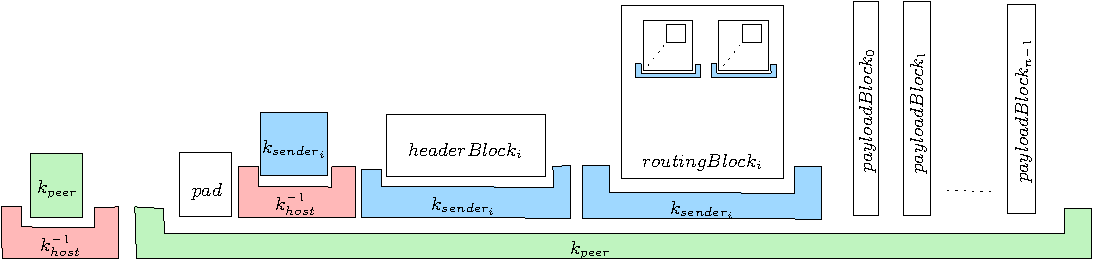
\includegraphics[width=\textwidth]{inc/blockLayoutSimplified}
	\caption{Simplified message outline}
	\label{fig:messageOutline}
\end{figure*}

Figure~\ref{fig:messageOutline} shows an outline of the block structure of a message destined to $host_o$. For a mathematical representation see figure~\ref{fig:mathMessage}.

The first block is the message prefix block $\mathbf{MP}$, which has been encrypted with the public key of the receiving node $K^1_{host_o}$. This block contains the key for decrypting the whole rest of the message. 

Immediately following the message prefix block, we have the inner message block. This message blocks contain four more blocks and is encrypted with the symmetrical peer key $K_{peer_o}$. This peer key is specific to this message and nowhere reused. It is only known by the two peer hosts $host_o$ and $host_{o-1}$, and the routing block builder (\defref{RBB}). More importantly, $host_{o-1}$ does not need to know the host key of $host_o$. Therefore, relaying a message to $host_o$ does not enable $host_{o-1}$ to communicate with $host_o$. 

The decryption key for the header block $\mathbf{HEADER}$ and the routing block $\mathbf{ROUTING}$ is obtained by $host_o$ from the header prefix block $HP$. After only decrypting the header block $\mathbf{HEADER}$ and verifying its signature, the accounting layer may check if further processing is authorized. 

After authorization, the header block is processed as outlined in section~\ref{sec:processingIncommingMessages}. Basically, we just add the routing blocks and payload to the respective workspace and wait for the routing layer to process the information.

Looking at a full \VortexMessage, we get the protocol outline, as shown in \eqref{eq:vortexMessage} on page~\pageref{eq:vortexMessage}.

\begin{figure*}[!ht]
	\begin{align}
	\mathbf{VORTEXMESSAGE}       = &\langle \mathbf{MP}^{K^{-1}_{hostN}}, INNERMESSAGE \rangle \label{eq:vortexMessage} \\ 
	\mathbf{INNERMESSAGE}        = &\langle \mathbf{CP}^{K^{-1}_{hostN}}, \mathbf{H}^{K_{senderN}}, E^{K^{-1}_{senderN}}\left(H\left(\mathbf{HEADER}\right)\right), \left[\mathbf{R}^{K_{senderN}}\right], \left[\mathbf{PL}\right]*\rangle^{K_{peerN}} \label{eq:innerMessage}\\
	\mathbf{MP}^{K^{-1}_{hostN}} = &E^{K^{-1}_{hostN}}\left(\mathbf{PREFIX}\langle K_{peerN}\rangle \right)\\ 
	\mathbf{HP}^{K^{-1}_{hostN}} = &E^{K^{-1}_{hostN}}\left(\mathbf{HPREFIX}\langle K_{senderN}\rangle \right)\\ 
	\mathbf{H}^{K_{senderN}}     = &E^{K_{senderN}}\left(\mathbf{HEADER}\right)\\  
	\mathbf{HEADER}              = &\langle K^{1}_{senderN}, serial, maxReplays, validity, [requests, requestRoutingBlock],\nonumber\\ 
	& [puzzleIdentifier, proofOfWork] \rangle \\  
	\mathbf{R}^{K_{senderN}}     = & E^{K_{senderN}}\left(\mathbf{ROUTING}\right)\\ 
	\mathbf{ROUTING}             = & \langle [ \mathbf{ROUTINGCOMBO} ] *, forwardSecret, replyBlock \rangle\\  
	\mathbf{ROUTINGCOMBO}        = & \langle processIntervall, K_{peerN+1}, recipient, \mathbf{nextMP}, \mathbf{nextHP}, \nonumber \\
	& \mathbf{nextHEADER}, \mathbf{nextROUTING}, assemblyInstructions, id \rangle\\
	\mathbf{PL}                  = &\langle \text{payload octets} \rangle *\\ 
	\end{align}
	%\captionsetup{labelformat=empty}
	\caption{Detailed representation of a VortexMessage}
	\label{fig:mathMessage}
\end{figure*}

The routing log block is an onionized block. It contains at least a $forwardSecret$, which must match up with the header blocks $forwardSecret$. This mechanism is required to guarantee that routing blocks are not exchanged. The $replyBlock$ provides a possibility, if provided, to contact the original sender of the message without knowing him. It is just a routing block with instructions on how to prepare the message to be sent. The routing combos contain all the necessary information and prebuilt blocks to create the subsequent messages.

At the very end, we got the payload. These blocks are simply added to the \defref{eID}s workspace.

The double encryption of the routing and header block, are doubly encrypted. We could argue that the inner message block should not be encrypted with a peer key. This looks like a flaw at first sight but is, in fact, a feature that is very important. Without this key, any independent observer with knowledge about the blending capabilities of a receiving node may\ldots
\begin{itemize}
	\item Easier to identify the block structure.\\ 
	This statement remains regardless of whether ASN.1 or length prefixed structures are used. If the structure of a \VortexMessage can be easily identified, the messages may be logged or dropped.
	\item Identify the routing block size.\\
	The value of this information is only minimal as it only reflects the complexity of the remaining routing information indirectly.
	\item Identify the number of payload blocks and their respective sizes. \\
	Sizing information is valuable when following the path of a message.
\end{itemize}

For the exact usage of the keys, see section~\ref{sec:keyUsage}.

\subsubsection{Message Structure Related to Censorship Circumvention}
It is important to note that there is no structure dividing the encrypted peer key from the Inner message block. The size of the peer key block is defined by the key and algorithm of the host key. 

The whole \VortexMessage is, looking from outside, a structureless blob with a maximum of entropy caused by the encryption employed. 

This is intentional and by design. Plain embedding uses furthermore a method of splitting, which allows a message block to be embedded in chunks in carrier information. By design, neither the message nor their embedding display detectable attributes allowing them to identify the message. 

Exactly as with the routing operations, great care has been applied. Any random sequence of bytes may be interpreted as valid chunking. For more exact implementation details on chunking, see section~\ref{sec:chunkingPlain}.

\subsubsection{Message Structure Related to Information Leaking}
From the inside, the $\mathbf{INNERMESSAGE}$ (see \ref{eq:innerMessage}) is built as structure leaking the absolute minimum of information.

\fxwarning{Missing content here (prio. 1)}

\subsection{Routing Operations}
The routing operations build the core as they define the capabilities of the mixing. We decided to introduce three different classes of operations. Unlike with the crypto algorithms, there is, at the current level, no flexibility when implementing those. We have not implemented any mechanism allowing us to replace these operations.

\subsubsection{$addRedundancy$ and $removeRedundancy$ Operations}
These operations build the core of the routing capabilities of a node. The operation allows a \defref{RBB} to add to a message redundancy information or to rebuild a block from a chosen set of information. 

The Operation itself is shown in figure~\ref{fig:addRedundancyOperation}. 
\begin{figure}[ht]\centering
	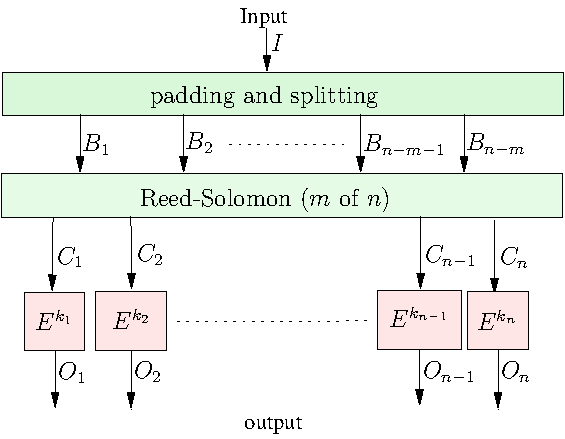
\includegraphics[width=0.8\columnwidth]{inc/addRedundancyOp}
	\caption{Outline of the addRedundancy operation}
	\label{fig:addRedundancyOperation}
\end{figure}

It may be subdivided into the following operations:
\begin{itemize}
	\item Pad the original message block in such a way, that all resulting blocks are a multiple of the block size of the encrypting cipher.
	\item Apply a Reed Solomon operation in a given GF space with a vanderMonde matrix.
	\item Encrypt all resulting blocks with unpadded, symmetrical encryption.
\end{itemize}

The padding applied in the first step is non-standard padding. The reason for this lies in the properties required by the operation. The presence of standard padding may leak, whether the block has been successfully decrypted or not. Therefore, we created a padding with the following properties:
\begin{itemize}
	\item The padding must not leak whether the rebuild cycle of the operation was successful or not.
	\item Anyone knowing the routing block content and the transmitted message must be able to predict any treated block, including all padding bytes.
	\item The padded content must provide resulting blocks of required size to enable non-padded encryption after the RS operation
	\item The padding must work with any size of padding space.
	\item The padded and encrypted block must not leak an estimate of the original content.
\end{itemize}

The padded block $\mathbf{X}$ is created from a padding value $p$, the unpadded block $\mathbf{M}$ and a series of padding bytes. We build $\mathbf{X}$ for a function $RS_{\text{m of n}}$ and an encryption block $\mathbf{M}$ sized $K$ as follows:
\begin{eqnarray}
i          & = & len(\mathbf{M})\\
e          & = & k \cdot n\\
l          & = & \left\lceil\frac{i + 4 + C2 }{e}\right\rceil\cdot e\\
p          & = & i + \left( C1 \cdot l \pmod{\left\lfloor\frac{2^{32}-i}{l}\right\rfloor\cdot l}\right)\\
\mathbf{X} & = & \langle p,\mathbf{M},R_{t}\left(s,l-i-4\right)\rangle
\end{eqnarray}    
The remainder of the input block, up to length $l$, is padded with random data. The random padding data may be specified by RBB though a PRNG spec $t$ and an initial seed value $s$. The message is padded up to size $L$. All resulting, encrypted blocks do not require any padding. This baecause the initial padding guarantees that all resulting blocks are dividable by the block size of the encrypting function. If not provided by an RBB, an additional parameter $C1$ is chosen as random positive integer and $C2=0$  by the node executing the operation.

To reverse a successful message recovery information the of a padded block $\mathbf{X}$, we calculate the original message size by extracting $p$ and doing $len(\mathbf{M})=p \pmod{ len(\mathbf{X})}$.

This padding has many important advantages:
\begin{enumerate}
	\item The padding does not leak if the rebuilding of the original message was successful. Any value in the padding may reflect a valid value.
	\item Since we have a value $C2$, the statement that a message size is within $len(\mathbf{X})<size<(len(\mathbf{X})-k\cdot n)$ is no longer true and any value smaller $len(\mathbf{X})-k\cdot n$ may be correct as well.
	\item An RBB may predict the exact binary image of the padded message when specifying $C1$, $C2$, and $R_{t}(s,)$.
	\item A node knowing the original parameters $C1$, $C2$, and the initial PRNG seed $s$ can detect successful decryption.
\end{enumerate}

Apart from being non-standard padding, the padding has additional downsides:
\begin{itemize}
	\item The padding is inefficient compared to simple paddings such as PKCS\#7
	\item The padding requires an initialized PRNG to generate the padding.
	\item Depending on the chosen parameters, the padding overhead may become significant. 
\end{itemize}

After the padding, the date is ready for the $addRedundancy$ operation. We first group the data vector into a matrix $\mathbf{A}$ with $m$ columns to do the operations efficiently. The previous padding guarantees that all columns have a length, which is dividable by the block size of the encryption step applied latter.

\begin{eqnarray}
t          & = & n-1\\
\mathbf{A} & = & vec2mat\left(\mathbf{X},\frac{len\left(\mathbf{X}\right)}{m}\right)\\
\mathbf{V} & = & \left(\begin{matrix}
0^0 & 0^1 & 0^2 & \cdots & 0^{(m-1)} \\
1^0 & 1^1 & 1^2 & \cdots & 1^{(m-1)} \\
2^0 & 2^1 & 2^2 & \cdots & 2^{(m-1)} \\
\vdots & \vdots & \vdots & \ddots & \vdots \\
t^0 & t^1 & t^2 & \cdots & t^{(m-1)}
\end{matrix}\right)\\
\mathbf{P} & = & \mathbf{V}\mathbf{A} \left(GF\left(2^\omega\right)\right)\\
\langle \mathbf{Q_1}, \ldots , \mathbf{Q_n} \rangle & = & row2vec(P)\\
R_i & = & E^{K_i}\left(Q_i\right)
\end{eqnarray}    

We do the Reed-Solomon operation by employing a Vandermonde matrix ($\mathbf{V}$). We build the data matrix ($\mathbf{A}$) by distributing the data into $\frac{len\left(\mathbf{X}\right)}{m}$ columns. This results in a matrix with $m$ rows. Unlike in error-correcting systems, we do not normalize the matrix so that the result of the first blocks is equivalent to the original message. Instead, the error-correcting information is distributed over all resulting blocks ($\mathbf{Q_i}$). Since the entropy of the resulting blocks is lowered as shown in figure~\ref{fig:entropy} and may thus leak an estimate of how a resulting block may have been treated, we added the encryption step to equalize entropy again. The previously introduced padding guarantees that there is no further padding on block-level required. The key used to encrypt the single blocks must not be equivalent. Equivalent keys have the side effect encrypting equal blocks into the same cyphertext. We observed faint but statistically relevant reminders of the unencrypted graphs when treating the same block with the same key and different redundancy parameters.

\section{Routing}
The routing layer receives the message blocks from the blending layer in a decrypted and authorized form and processes them as follows:

\begin{itemize}
	\item Build structure representing the block building and the appropriate block IDs.
	\item Schedule all Routing blocks for processing in a priority queue.
	\item Authorise all routing blocks ready for processing with the calculated block sizes.
	\item Process blocks.
	\item Send prepared building blocks to the Blending Layer.
\end{itemize}

\subsubsection{$encrypt$ and $decrypt$ Operations}
The encrypt and decrypt operations are essential for the requirement that tagging should not be possible. Unlike the $addRedundancy$ and $removeRedundancy$, the splitting operations do not feature any encryption step after splitting or merging. Reusing a payload block that has only been split or merged would repeat the payload pattern on multiple nodes during transfer. That is why we require to have encryption.

The reason for not building this step into the split and merge function was simple. We needed a separate encryption step to be able to work as an onionizing system, and there were use cases where integrated encryption did not make sense. For further details on this topic, see section~\ref{sec:routingStrategies}.


\subsubsection{$mergePayload$ and $splitPayload$ operation}
The $splitPayload$ operation splits a payload block into two chunks of different or equal sizes. The parameters for this operation are:

\begin{itemize}
	\item source payload block $pb_1$
	\item fraction $f$\\
	A floating-point number which is describing the size of the first chunk. If the fraction is ``1.0'', then the whole payload is transferred to the second target chunk
\end{itemize}

If $len(pb_1)$ expresses the size of a payloadblock called $pb_1$ in bytes then the two resulting blocks of the SpitPayload Operation $pb_2$ and $pb_3$ have to follow the following rules:

\begin{eqnarray}
split(f, pb_1) & = &\langle pb_1, pb_2 \rangle\\
pb_1.startsWith(pb_2)\\
pb_1.endsWith(pb_3)\\
len(pb_2) & = & floor(len(pb_1)\cdot f)\\
len(pb_1) & = & len(pb_2) + len(pb_3)
\end{eqnarray}

The $mergePayload$ operation combines two payload blocks into one. The parameters for this operation are:

\begin{itemize}
	\item first source payload block $pb_1$
	\item second source payload block $pb_2$
\end{itemize}

If $len(pb)$ expresses the size of a payloadblock called $pb$ in bytes then resulting block of the MergePayload Operation $pb_3$ have to follow the following rules:

\begin{eqnarray}
merge(pb_1, pb_2) & = & pb_3 \\
pb_3.startsWith(pb_1)\\
pb_3.endsWith(pb_2)\\
len(pb_3) & = & len(pb_1) + len(pb_2)
\end{eqnarray}

Unlike other operations, this operation has no encryption step attached to it. We usually attached an encryption step to remove repeating patterns from the \VortexMessage stream

It has to be mentioned that this operation tuple has some issues when it comes to floating-point implementations. They are solvable but had to be specified unexpectedly precisely in order to enable a true cross-platform implementation. For more information regarding the issue and exact implementation, see section~\ref{sec:implOperations}.

\subsection{Key Usage\label{sec:keyUsage}}
The key usage is essential for \MessageVortex. For authentification and transmission of the session keys ($K_{sender_o}$ and $K_{peer_o}$), we use long living asymmetrically built keys. These keys remain, once chosen and distributed statically in the system. This leads directly to the problem of key distribution within our system. This concern is addressed in section~\ref{sec:keyDistribution}.

To round up findings: We must distribute all keys not 


%\section{TBI:Vortex Communication model}
%In this section, we introduce a new consistent, transport-independent model for representing the different protocols used by MessageVortex.
%
%\begin{figure}[ht!]
%    \centering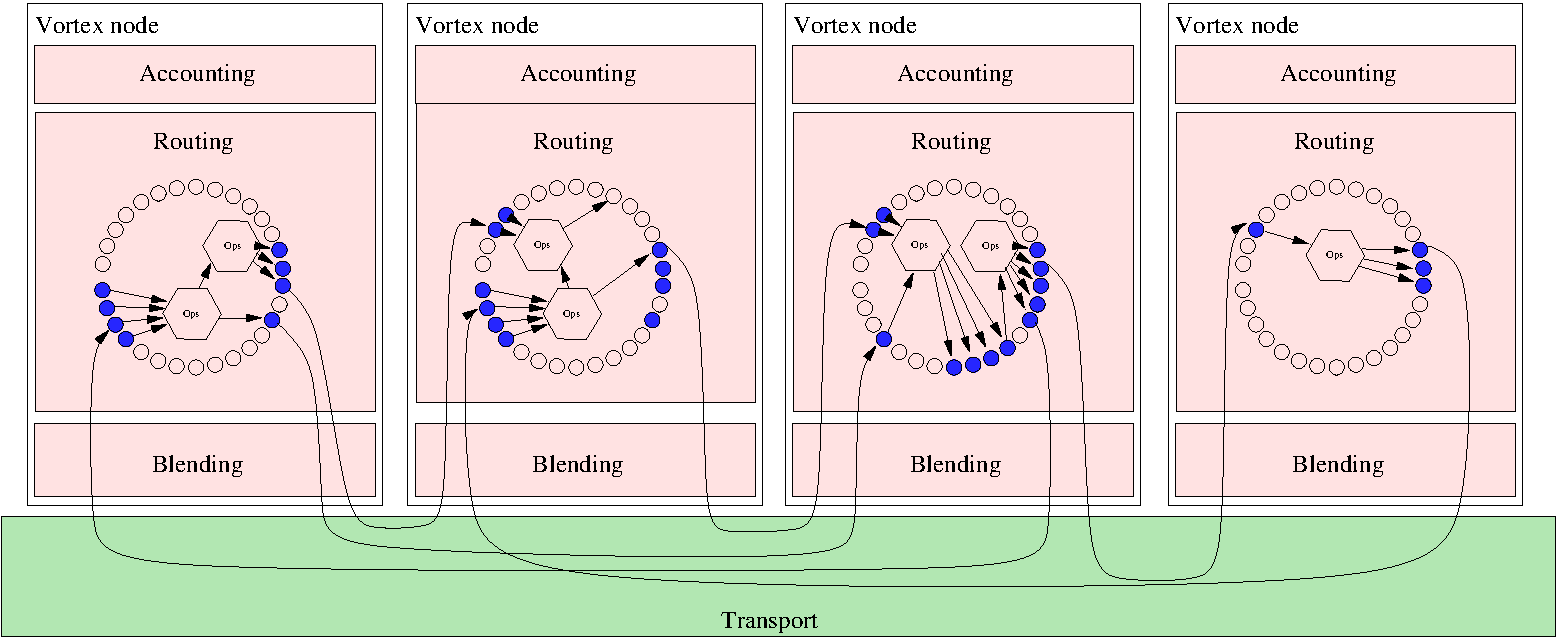
\includegraphics[width=\columnwidth]{inc/roughProtocolDesign.pdf}
%    \caption{A rough protocol outline of the MessageVortex protocol}\label{fig:protocolOutline}
%\end{figure}
%
%We divide our protocol into four different layers, whereas only three are specific to the MessageVortex protocol. The lowest layer is the transport layer. As expressed earlier, dedicated protocols are easy to censor. Therefore we build our protocol on top of other suitable transport protocols. 
%
%The other Three layers are vortex specific and do not require any infrastructure on the Internet. We elaborate further on these layers in the next section.
%
%\section{TBI:Protocol handling}
%In the following sections, we outline the handling of messages we split the handling into incoming messages and outgoing messages. All handling assumes that we have a blending layer independently picking up messages as advertised in the capabilities messages.
%

